\subsubsection{Energieversorgung}
\label{subsubsec:energieversorgung}

In der Abbildung \ref{fig:Energieversorgung} ist die Systemgrenze (gestrichelte Linie) der mobilen Wetterstation ersichtlich. Innerhalb dieser Systemgrenze befinden sich der \textit{Akkumulator}, der \textit{MCP73871} Ladechip, der \textit{LM1117} 3.3V Linearregler und der \textit{LMC7660} Spannungswandler. Ausserhalb der Systemgrenze sind die Photovoltaikanlage, rsp. das Solarpanel, das 230V AC-Stromnetz und ein Computer. Das Solarpanel, sowie auch das Stromnetz können über einen DC Jack Stecker mit den Dimensionen 5.5mm Aussen- und 2.1mm Innendurchmesser angeschlossen werden. Zusätzlich ist der Akkumulator ebenfalls über den USB 2.0 micro-B Anschluss mittels Computer ladbar. Somit kann die Wetterstation auch bei ungenügender Sonneneinstrahlung geladen werden. Es ist möglich, beide Anschlüsse gleichzeitig angeschlossen zu haben.\\

\begin{figure}[h]
	\centering
	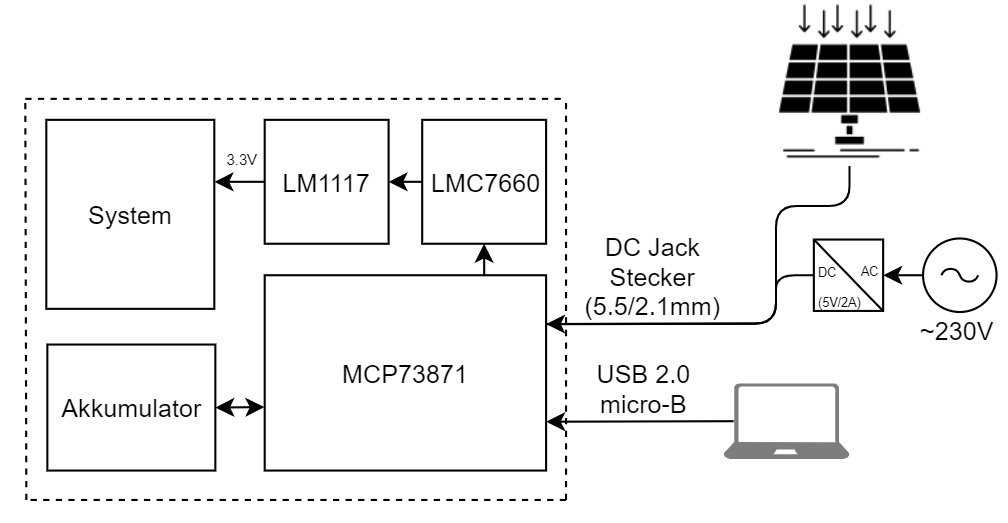
\includegraphics[scale=0.5]{graphics/Konzeptdiagramme/Energieversorgung.PNG}
	\caption{Energieversorgung}
	\label{fig:Energieversorgung}
\end{figure}

Der \textit{Akkumulator} bildet das Kernstück der Energieversorgung, da dieser die Quelle für die mobile Wetterstation ist. Er dient als Stützung der Versorgungsspannung (3.3V), falls die Wetterstation nur über das Solarpanel betrieben wird, damit sie auch in der Nacht funktionstüchtig bleibt. Der \textit{MCP73871} ist der Ladechip. Dieser reguliert den Ladestrom in Abhängigkeit des Laststromes vom System. Damit der \textit{LM1117} konstant 3.3V als Systemspannung generieren kann, wird der \textit{LMC7660} als positiver Spannungsmultiplizierer vorgeschaltet. Der Funktionsblock \textit{System} beinhaltet alle Bauteile der Wetterstation, welche mit 3.3V Versorgungsspannung betrieben werden müssen. Da die Wetterstation auf Low Consumption ausgelegt wird, sind dies fast alle Bauelemente.\\
 